\documentclass[10pt,twocolumn,letterpaper]{article}




\usepackage{cvpr}
\usepackage{times}
\usepackage{epsfig}
\usepackage{graphicx}
\usepackage{amsmath}
\usepackage{amssymb}



% Include other packages here, before hyperref.

% If you comment hyperref and then uncomment it, you should delete
% egpaper.aux before re-running latex.  (Or just hit 'q' on the first latex
% run, let it finish, and you should be clear).
\usepackage[pagebackref=true,breaklinks=true,letterpaper=true,colorlinks,bookmarks=false]{hyperref}

\cvprfinalcopy % *** Uncomment this line for the final submission

\def\cvprPaperID{****} % *** Enter the CVPR Paper ID here
\def\httilde{\mbox{\tt\raisebox{-.5ex}{\symbol{126}}}}

% Pages are numbered in submission mode, and unnumbered in camera-ready
\ifcvprfinal\pagestyle{plain}\fi
\begin{document}


%%%%%%%%% TITLE
\title{The Hateful Memes Challenge: Detecting Hate Speech in Multimodal Memes\\  CS 7643}

\author{Jisheng Chen, Yao Xu, Guolin Yao\\
Georgia Institute of Technology\\
% Institution1 address\\
{\tt\small jishengchen3120@gatech.edu, yxu632@gatech.edu, gyao30@gatech.edu }
}
% For a paper whose authors are all at the same institution,
% omit the following lines up until the closing ``}''.
% Additional authors and addresses can be added with ``\and'',
% just like the second author.
% To save space, use either the email address or home page, not both
% \and
% Second Author\\
% Institution2\\
% First line of institution2 address\\
% {\tt\small secondauthor@i2.org}
% }

\maketitle
%\thispagestyle{empty}

%%%%%%%%% ABSTRACT
\begin{abstract}
  The urgency of detecting hate speech in memes comes from a combination of increasing hate speed on social media and lacking effective machine learning tools to identify/stop them. Detecting hate speech in memes is challenging for AI as it requires reasoning about subtle cues in a multimodal setting (e.g., image and text). The Current state-of-the-art (SOTA) multimodal models perform much poorer compared to human performance (64.73\% vs. 84.7\% accuracy), indicating that there is much room for research and improvement. The goal of this project is to construct some multimodal models to improve the hate speech detection task. To this end, we replicated the Facebook multimodal pre-trained baselines: Visual BERT and Visual BERT COCO; then we further replicated the third winner’s solution which is applying grown training set, extracting image features using Detectron algorithm, fine-tuning pretrained Visual BERT model; and finally we removed the text from the image and applied the object detection (Detectron) algorithm to explore how different feature extraction affect the performance of the models. In this report, we document our experiments and challenges, describe our model setups, report our implementation and validation results and compare them to SOTA model performance, finally, discuss and interpret our findings.
\end{abstract}

%%%%%%%%% BODY TEXT
\section{Introduction/Background/Motivation}

As malicious contents exploded on the internet, it is almost infeasible for humans to detect them manually. Instead, creating an artificial intelligence/machine learning system to recognize those harmful speeches becomes imperative to prevent them from spreading when mitigating important societal problems. For example, preventing hate speech from widely spreading on the internet could potentially avoid real-world violence.
 
The hateful memes challenge from Facebook is challenging mainly due to the nature of the problem, which is multimodal involving both language and image confounders. In a unimodal language setting, sentences such as “Look at how many people love you” or “Love the way you smell today” may seem to be harmless, but when combining them with an equally harmless image of a tumbleweed or skunk, the sentences will suddenly become mean and hateful (Figure \ref{fig:illustration}). While the underlying meanings of those memes are easy for humans to understand, they can be very challenging for AI systems, especially for those with unimodal reasoning. One of the most important characteristics in this challenge is that “benign confounder” is introduced to underperform the models with unimodal priors. More specifically, it exits alternative images or captions in the dataset that make the label flip from hateful to not-hateful or vice versa. Take the skunk’s image with text “Love the way you smell today” as an example, if we change the image to rose, or change the caption to “Love the way skunk smell”, the memes will become harmless. As a result, the challenge can only be solved successfully by sophisticated multimodal reasoning and understanding. 

Current approaches for identifying hateful multimodal include unimodal models such as BERT, XLM-R, Roberta, multimodal models such as BERT + Resnet that were unimodally pretrained, and multimodal models that were multimodally pretrained such as VisualBERT and ViLBERT. The SOTA models for this problem are MMBT, ViLBERT, and VisualBERT, of which VisualBERT yields the best performance on the baseline model pre-trained on COCO Captions. The VisualBERT model is pre-trained using self-supervised pre-training proxy-tasks and fine-tuned on Hateful Memes dataset. 



\graphicspath{ {./images/} }

\begin{figure*}
\begin{center}
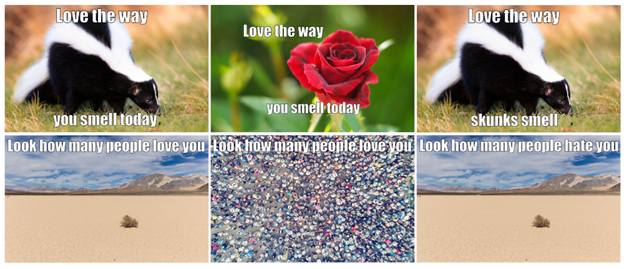
\includegraphics[scale = 1]{Figure1}
% \fbox{\rule{0pt}{2in} \rule{.9\linewidth}{0pt}}
\end{center}
   \caption{Picture illustration of multimodal memes and benign confounders \cite{g_kiela2021hateful}}
\label{fig:illustration}
\end{figure*}

VisualBERT, which consists of a stack of Transformer layers that implicitly align elements of an input text and regions in an associated input image with self-attention (Figure \ref{fig:encoder}), is a simple and flexible framework for modeling a broad range of vision-and-language tasks. Research shows that VisualBERT can outperform or rival SOTA models in various tasks including VQA, VCR, NLVR, and Flickr30K while in the meantime, keeps a much simpler structure. The core idea of VisualBERT is to reuse the self-attention mechanism within the Transformer to implicitly align elements of the input text and regions in the input image \cite{b_li2019visualbert}\cite{a_vaswani2017attention}. It adds a set of visual embeddings F to BERT, which can model an image and each f to F corresponding to a bounding region in the image, derived from an object detector. 

The input representation of VisualBERT includes following: 1) tokenize the given word into word pieces, and a token embedding is related to each of the subword, 2) segment embedding, indicating which part of text the token comes from (e.g., the first or second sentence), 3) a position embedding indicating the position of the word in the sentence. A similar structure of the 3 embeddings will be constructed from the image as well: 1)  a visual feature representation of the bounding region computed by a CNN, 2) a segment embedding indicating it is an image embedding as opposed to a text embedding, and 3) a position embedding  which is used when alignments between words and bounding regions are provided as part of the input, and set to the sum of the position embeddings corresponding to the aligned words (Figure \ref{fig:architecture}). Both visual embeddings and text embeddings are passed to the multi-layer Transformer,  allowing the model to implicitly discover useful alignments between both sets of inputs, and build up a new joint representation \cite{b_li2019visualbert}.

The hateful memes dataset is downloaded from DRIVENDATA. It contains 12540 images in total, of which 8500 are training set, 1500 are validation set and 2540 are test set. Only 12140 are unique images, and 400 are replicated in the validation datasets. The hateful memes dataset consists of 40\% multimodal hate, 10\% unimodal hate, 20\% benign text confounder, 20\% benign image confounder, 10\% random non-hateful \cite{g_kiela2021hateful}. Two types of efforts have been tried to augment the data: 1) searching for open-source dataset online, and 2) using the third winner’s Memotion dataset. Unfortunately, few relevant dataset were found online; many images in the Memotion dataset are wrongly labeled \cite{e_velioglu2020detecting}, and the number of images ($ \sim $14K) in the Memotion dataset 
is too small to improve the results. Therefore, we decided to stay with the original dataset (12540 images).

\begin{figure}[t]
\begin{center}
% \fbox{\rule{0pt}{2in} \rule{0.9\linewidth}{0pt}}
   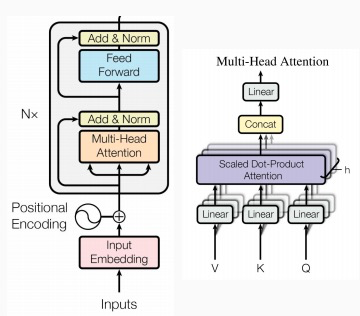
\includegraphics[width=1 \linewidth]{Figure2.png}
\end{center}
   \caption{Encoder unit and multi-headed self-attention structure used in VisualBERT \cite{a_vaswani2017attention}}
% \label{fig:long}
\label{fig:encoder}
\end{figure}

\begin{figure*}
\begin{center}
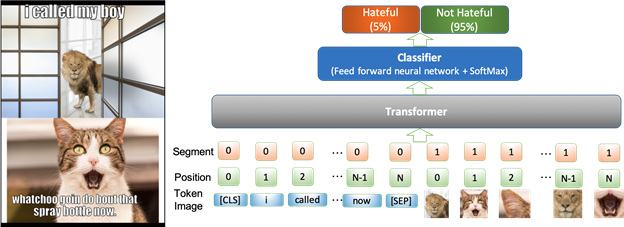
\includegraphics[scale = 1]{Figure3}
% \fbox{\rule{0pt}{2in} \rule{.9\linewidth}{0pt}}
\end{center}
   \caption{The architecture of VisualBERT. Image regions and languages are combined and then passed to a Transformer to allow the self-attention to discover implicit alignment between language and vision.}
\label{fig:architecture}
\end{figure*}
% \subsection{Miscellaneous}
%------------------------------------------------------------------------
% \subsection{Formatting your paper}

%  \href{https://arxiv.org/abs/1803.09010}{here}. You don’t have to choose all of them, just the most relevant.
%-------------------------------------------------------------------------
%------------------------------------------------------------------------
\section{Approach}
Our approach to this problem can be divided into two parts: the first part is to reproduce the baseline multimodal models \cite{g_kiela2021hateful} and the solution from the third winner in Hateful Memes Challenge \cite{e_velioglu2020detecting}; the second part is to apply ablation method to investigate the effects of different variables on the performance of the multimodal models, i.e., learning rate, image encoders, pre-trained multimodal models, data preprocessing, etc. Specifically, for the baseline replication, we choose the models pre-trained by ViLBERT CC and VisualBERT COCO) to have a sense of how SOTA models behave and get familiar with a vision-language multimodal framework (MMF) provided by Facebook AI Research (FAIR). When studying the solution from the third winner, we found they applied to their final submission the grown training set, extracting image features using Detectron algorithm, fine-tuning pre-trained VisualBERT model, hyperparameters sweep, and ensemble learning with majority voting techniques. The complexity of their work is beyond our goal for the current project due to the time and computation limitation. Therefore, to simplify our model, we only replicate the results from their first submission which did not use hyperparameters sweep and ensemble learning with majority voting . Take these replications as a starting point, we modify different parameters to conduct the experiments for the multimodal model training.

\subsection{Data Pre-processing}
Since the texts for model training have been extracted and are ready for use, it is not necessary to use Optical Character Recognition (OCR) to recognize and extract the texts again. Yet, the solution from the top winner in the competition \cite{f_zhu2020enhance} used OCR and inpaint model to find and remove the text from the image and the results showed improvement in the quality of object detection and web entity detection. Following this idea, we simplified the image pre-processing method by using OCR only to generate the clean meme image and then fed the images to the image encoder, aiming at seeing how this pre-processing could affect the model performance. Figure \ref{fig:sample} shows a sample image from the hateful memes dataset before and after OCR pre-processing.

\begin{figure}[t]
\begin{center}
% \fbox{\rule{0pt}{2in} \rule{0.9\linewidth}{0pt}}
   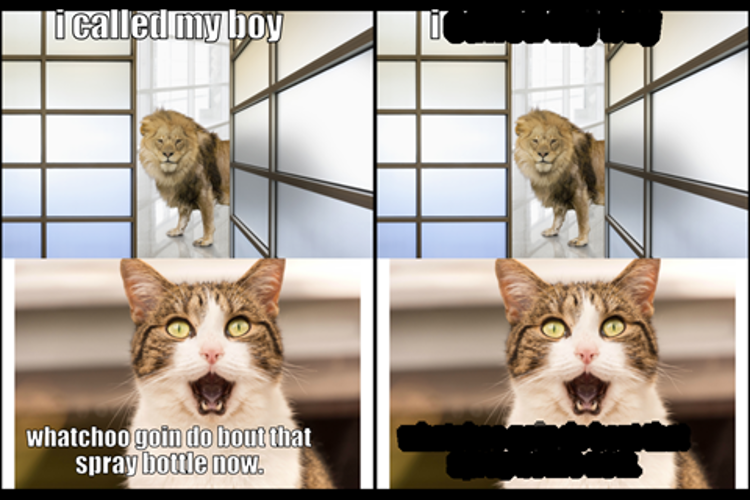
\includegraphics[width=1 \linewidth]{Figure4.png}
\end{center}
   \caption{ Sample mages before (left) and after (right) OCR pre-processing.  ©Getty Images}
% \label{fig:long}
\label{fig:sample}
\end{figure}
% \textbf{Important: Mention any code repositories (with citations) or other sources that you used, and specifically what changes you made to them for your project. }

\subsection{Feature Extraction}
In a multimodal model, the extracted image features and textual features are combined to classify hateful memes. FAIR has provided a powerful framework (Detectron) for object detection and instance segmentation. An object detection model in Detectron, employing a fc6 layer of Mask R-CNN with Resnet152 as its backbone network architecture, is used to collect 100 bounding boxes of region-based image features per image in this project. As described in Figure \ref{fig:architecture}, the visual embeddings are projected into the textual embedding space before passing them through the transformer layers. The first output of the final layer in the model is used as the input to a classifier. The classification layer can be defined as cls(\textit{x}) = \textit{Wx} + \textit{b}, where the dimension of weights \textit{W} is \textit{D} * \textit{C}  (\textit{D} is transformer dimensionality and \textit{
C} is the number of classes) \cite{e_velioglu2020detecting}. Softmax activation function is applied to the final logits to output the predicted probability. We also apply another object detection model which uses Mask R-CNN with Resnet101 as its backbone architecture to investigate the effect of different object detectors on the performance of the multimodal model. 

\subsection{Model Selection}
As described above, the hateful memes dataset including difficult examples is designed to tackle the task with multimodal techniques, which make it hard to purely rely on unimodal signals. To achieve an improved performance of the model, two pre-trained multimodal models (ViLBERT CC and VisualBERT) are selected as the starting models and fine-tuned using different parameters. VisualBERT is originally pre-trained on COCO image caption dataset, but the results by Velioglu and Rose \cite{e_velioglu2020detecting} showed that the model pre-trained on Conceptual Captions obtains better scores. Also, the two models are SOTA baseline models which achieve the highest area under the receiver operating characteristic curve (AUROC) and accuracy among all the models. Therefore, we perform different experiments with these two models based on MMF. 

\section{Experiments and Results}
\subsection{Overview, Measurements, and Baselines}
In light of the requirement in the hateful memes challenge, we adopted accuracy and AUROC to evaluate the performance of the models. Accuracy is to evaluate the proportion of data that are correctly labeled. AUROC is widely used to evaluate performance of classification problems. It measures the model’s capability of distinguishing between classes with higher values indicating better performance. An AUROC of 0.7 means that 70\% of the time, the model will correctly assign the “hateful” label to a randomly selected “hateful” image than to a randomly selected “non-hateful” image.
 
We first replicated three baseline models to check the “settings” of our models: ViLBERT CC and VisualBERT COCO provided by Facebook \cite{d_kiela2021hateful} and VisualBERT COCO tuned and trained by the third winner \cite{e_velioglu2020detecting} (Table \ref{tab:replication}). Our replication results are very close to the original results provided by Facebook and the third winner, confirming the validity and feasibility of our model settings.

Our efforts of improving the model performance are primarily from five aspects: 1) the choice of model (Experiment 2 (E2) and E6, E11 and E12  in Table \ref{tab:summary}), 2) variations in learning rate (E1-5), 3) different image encoders (E2 and E8, E9 and E12), 4) changes in batchsize (E6 and E7), and 5) the prep-rocessing treatments of datasets (E5 and E10, E8 and E9, E2 and E12). Table \ref{tab:summary} summarizes the model performance of different experiments. The rest of the result sections will discuss the results from these five aspects in detail.

%-------------------------------------------------------------------------
\begin{table*}
\begin{center}
\begin{tabular}{c|c|c|c|c}
\hline
& \multicolumn{2}{c}{Replication results} & \multicolumn{2}{c}{Original results} \\
\hline\hline
Model Name & Accuracy & AUROC & Accuracy & AUROC \\ \hline
VilBERT CC (Baseline) & 67.96 & 66.01 & 61.40 & 70.07 \\ \hline
Visual BERT COCO (Baseline) & 67.04 & 69.96 & 65.06 & 73.97 \\ \hline
Visual BERT COCO (3rd sub1) & 73.52 & 75.68 & 70.93 & 75.21 \\ \hline
\end{tabular}
\end{center}
\caption{Replications of the baseline models.}
\label{tab:replication}
\end{table*}
%-------------------------------------------------------------------------

%-------------------------------------------------------------------------
\begin{table*}
\begin{center}
\begin{tabular}{c|c|c|c|c|c|c|c}
\hline
No. & Model & Learning rate & Image encoder & Batch size & Dataset & Accuracy & AUROC \\
\hline\hline
1 & Visual BERT COCO & 0.001 & Mask R-CNN + ResNet-152 & 32 & OCR pre-processed & 67.96 & 72.31 \\
\hline
2 & Visual BERT COCO & 0.01 & Mask R-CNN + ResNet-152 & 32 & OCR pre-processed & 67.59 & 71.39 \\
\hline
3 & Visual BERT COCO & 0.05 & Mask R-CNN + ResNet-152 & 32 & OCR pre-processed & 70.93 & 73.98 \\
\hline
4 & Visual BERT COCO & 0.1 & Mask R-CNN + ResNet-152 & 32 & OCR pre-processed & 67.78 & 72.95 \\
\hline
5 & Visual BERT COCO & 0.3 & Mask R-CNN + ResNet-152 & 32 & OCR pre-processed & 70.00 & 74.02 \\
\hline
6 & ViLBERT CC & 0.01 & Mask R-CNN + ResNet-152 & 32 & OCR pre-processed & 62.20 & 71.61 \\
\hline
7 & ViLBERT CC & 0.01 & Mask R-CNN + ResNet-152 & 16 & OCR pre-processed & 69.07 & 68.54 \\
\hline
8 & Visual BERT COCO & 0.01 & Mask R-CNN + ResNet-101 & 32 & OCR pre-processed & 64.00 & 69.59 \\
\hline
9 & Visual BERT COCO & 0.01 & Mask R-CNN + ResNet-101 & 32 & RAW & 61.00 & 66.98 \\
\hline
10 & Visual BERT COCO & 0.3 & Mask R-CNN + ResNet-152 & 32 & RAW & 69.63 & 73.91 \\
\hline
11 & ViLBERT CC & 0.01 & Mask R-CNN + ResNet-152 & 32 & RAW & 70.15 & 72.63 \\
\hline
12 & Visual BERT COCO & 0.01 & Mask R-CNN + ResNet-152 & 32 & RAW & 72.96 & 75.65 \\
\hline
\end{tabular}
\end{center}
\caption{A summary comparisons of model performance of different experiments.}
\label{tab:summary}
\end{table*}
%-------------------------------------------------------------------------

\subsection{Learning Rates}
Learning rate is a hyperparameter in the gradient descent to control the “converging” speed. A large learning rate can accelerate converging speed but could also miss the optimal point. A small learning rate is not likely to miss the optimal point but could be costly and slow. Using VisualBERT COCO model with a Mask R-CNN + ResNet-152 image encoder on the OCR pre-processed dataset, we tested learning rates of [0.001, 0.01, 0.005, 0.1, 0.3] (E1-5 in Table \ref{tab:summary}) and evaluated their effects on the model performance (Figure \ref{fig:lr}). Model performance generally improves as the number of iterations increases. The learning rate of 0.001 denoted in blue line has slightly worse performance compared to other learning rates at higher iterations due to the slow converging speed. As the learning rate is greater than 0.01, it is challenging to conclude a certain relationship between the model performance and the learning rate. In this particular case, the learning rate of 0.05 (denoted by green line) performs slightly better than other learning rates.


\begin{figure}[t]
\begin{center}
% \fbox{\rule{0pt}{2in} \rule{0.9\linewidth}{0pt}}
   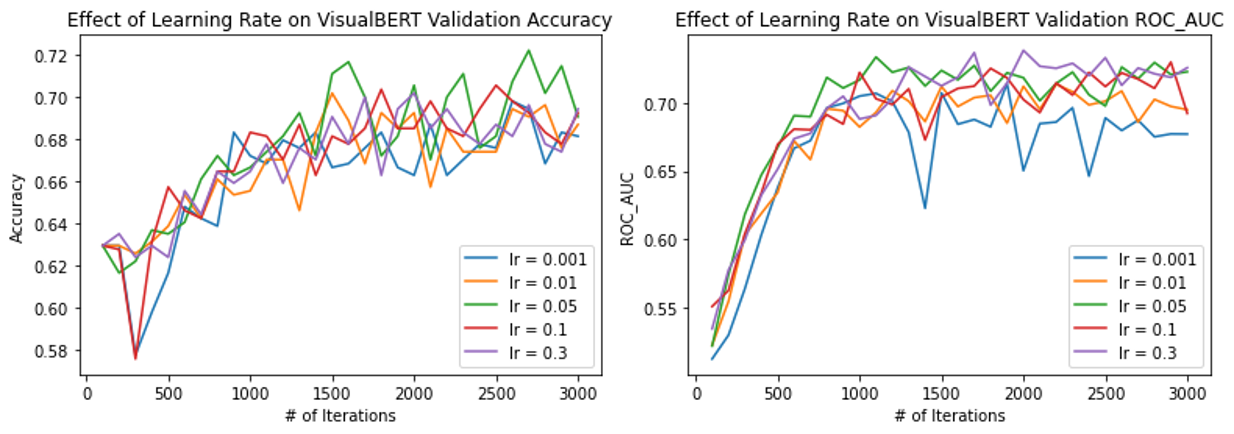
\includegraphics[width=1 \linewidth]{Figure5.png}
\end{center}
   \caption{The effects of learning rates on VisualBERT performance}
% \label{fig:long}
\label{fig:lr}
\end{figure}


\subsection{Batch Size}
Batch size is the number of training examples in one iteration. Keskar et al. \cite{h_keskar2017largebatch} found that a smaller batch size has faster training speed and better generalization capability in deep learning, as the larger-batch models might converge to “sharp minimizers” of the training function. Similar comparisons have been discussed by Andrew Ng: computing gradient descent on the entire dataset (an extreme case of large batch size) may be the “best” leading to the local minima but is highly expensive, while computing gradient descent on 1 training example (an extreme case of small batch size) may lead to a wrong direction but is fast. However, training on the entire dataset could lead to “overfitting” while training on one example could be too small to lead to a good local minima \cite{i_Authors14}. In this project, we tested two different bath sizes (16 and 32) on ViLBERT CC with Mask R-CNN + ResNet-152 image encoder and a learning rate of 0.01 on the OCR pre-processed dataset (E6 and E7 in Table \ref{tab:summary}). A batch size of 16 has higher accuracy than batch size 32 but lower AUROC. However, the computation costs (time and space) of a batch size of 16 is significantly lower than a batch size of 32 in this case. Without sacrificing the model performance, a batch size of 16 (a relatively smaller batch size) is thus preferred. 

\subsection{Image Encoders}
One of the highlights of this project is to apply different image encoders to extract image features. ResNet 152 \cite{i_Authors14b} and ResNet 101 \cite{i_Authors14c} are deep residual learning networks for image recognition. Image recognition ability is rewarding by adding more layers to the ResNet model but higher computation costs. Our results ((E2 and E8, E9 and E12 in Table \ref{tab:summary}; Figure \ref{fig:resnet}) further confirm this insight showing that ResNet152 has better performance than ResNet101.

\begin{figure}[t]
\begin{center}
% \fbox{\rule{0pt}{2in} \rule{0.9\linewidth}{0pt}}
   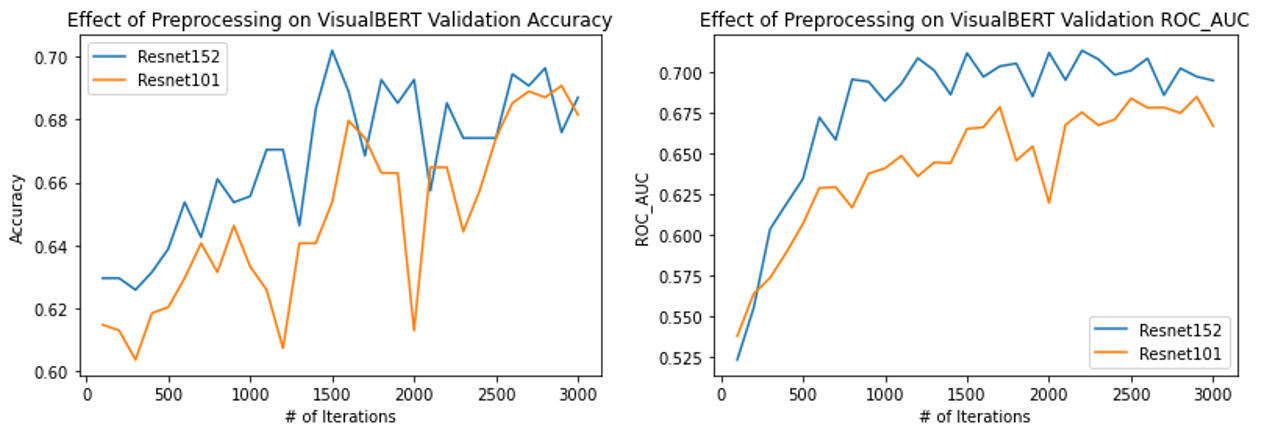
\includegraphics[width=1 \linewidth]{Figure6.png}
\end{center}
   \caption{The effects of ResNet152 and ResNet101 on VisualBERT performance}
\label{fig:resnet}
\end{figure}


\subsection{Preprocessing Dataset vs. Original Dataset}
Inspired by the top winner, the most important highlight of this paper is to use OCR to pre-process the images, which is to find and remove text captions on the image and avoid confusions in image recognition. We expect a better performance by preprocessing the dataset with OCR (E5 and E10, E8 and E9, E2 and E12 in Table \ref{tab:summary}; Figure \ref{fig:ocr}) but observe the opposite in most cases (except for E5 and E10 which have similar performance). One possible reason is that OCR pre-processing blacked the areas with texts and some image information is possibly lost in this process. Moreover, compared to the pre-processing method from the top winner, our method only considered OCR pre-processing without using inpant model, which could also be the reason that the pre-processing has the opposite effect to the top winner's solution. Nonetheless, it is a good practice to pre-process the images and test the effects of OCR treatment of the dataset.

\begin{figure}[t]
\begin{center}
% \fbox{\rule{0pt}{2in} \rule{0.9\linewidth}{0pt}}
   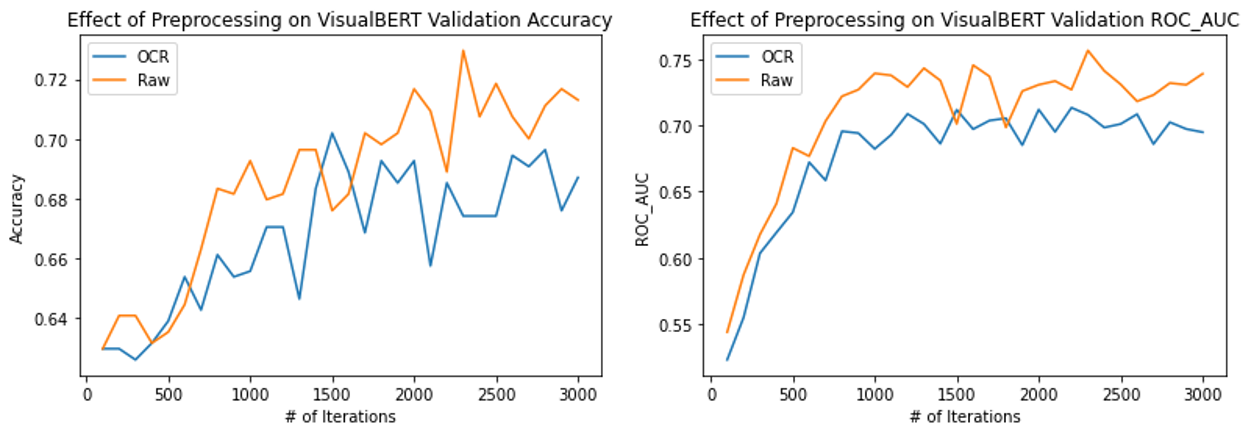
\includegraphics[width=1 \linewidth]{Figure7.png}
\end{center}
   \caption{The effects of OCR preprocessing on VisualBERT performance}
\label{fig:ocr}
\end{figure}


\subsection{VisualBERT COCO vs. ViLBERT CC}
VisualBERT COCO and ViLBERT CC are two multimodal baseline models with multimodal pre-training. In the baseline results provided by Facebook, VisualBERT COCO performs better than VilBERT CC, and many teams, such as the third winner, found that VisualBERT COCO yields the best performance. We tested the choice of the two models in our settings (E2 and 6, E11 and E12 in Table \ref{tab:summary}). Better performance of VisualBERT COCO still holds for both OCR pre-processed dataset and raw dataset. 

\subsection{Overfitting}
Overall the model works well on the unseen validation dataset with both accuracy and ROC higher than 0.7, which is very similar to the results in the training dataset, indicating no overfitting and well generalizability of the model. However, we did observe that when the training epoch keeps increasing, the performance of the final model slightly decreased compared to the best model we saved as checkpoint during the training process. It’s intuitive that the model will overfit with unnecessary long training epochs, therefore, we only kept the “best” model identified via validation, and used it for future prediction. As a result, the final models generalized well on the validation dataset, the accuracy/AUROC values were similar in both training and validation sets. 

\section{Experience}
\subsection{Cloud Computation}
We have encountered several challenges when working on cloud computation for this project. Due to the limited credits for Google Cloud Platform (GCP), we firstly started our project on Google Colaboratory (Colab). However, Google Colab has restrictions on the resources and time of free users. The default disk space allowed to use is only 28G. When a lot of packages are installed, there is not much space left. This is extremely limited especially when we were performing feature extraction and model training, which could generate lots of large size files. More importantly, the disk space provided by Google Colab is temporary. When the connection is disconnected, all files will be lost and we'll need to re-start the whole process. In the meantime, we need to store all data files in our own google drive network disk during the whole process of the project, which requires large storage space in google drive. Fortunately, one of our teammates has an unlimited storage google drive account which can be used to tackle this problem. Another limitation in Google Colab is the use of time when running GPU. The time restriction on running GPU (random) in Google Colab is stricter than that on running CPU (12h). Based on our experience, we found our computations have been suspended several times randomly because of running GPU for a time duration (2$ \sim $6h). After the suspension, we have to wait for at least 12 hours until we can use it again. Besides, Google Colab is an interactive platform that needs the user to be active during the usage, it will disconnect automatically if no user activity on the page for a short period of time. This is difficult to maintain especially when we were extracting the image features or training the model longer than 6 hours. As a result, we resorted to a window actively clicking method to solve the problem. After several successful trials of our training models on Google Colab, we started to transfer our model to GCP. Since we are all new to GCP, this process also took us longer than expected. The difficulties include building the connection to activate Jupyter Notebook, setting multi-thread layer GPU environment, and debugging when using MMF on GCP.

\subsection{Feature Extraction}
We solved several problems during image feature extraction: 1) To deal with the space limit, we specified an image range (2000 images at a time) to be extracted instead of extracting all at once. But this treatment led to two additional issues. Firstly, the range index specified by the MMF arguments did not follow the increasing order strictly. For instance, when running two sections for ranges [0,2000] and [2001, 4000], it was found that the number of the extracted feature files was not equal to the sum of two ranges, which indicates that there were some unknown duplicate operations during the extraction, and extra processing was necessary to cover the whole dataset. Secondly, the file storing between Google Colab and Google Drive was inconsistent. Part of files could be lost even though those files have been set to be saved in a permanent google drive. To tackle these two issues, we found out the lost images, re-fed them to the feature extractor, and finally achieved all the image features. 2) The second challenge comes from how to correctly configure MMF packages. Despite MMF offers different powerful packages to realize various functions, the tutorials are not very clear. We have to read the source codes to figure out what exactly the bugs came from and modify the source codes correspondingly. For example, MMF required specific image format and the raw images should be converted to that format and stored in a specific cache folder. The folder should be named following their definition, and the required image format should be .jpg (hateful memes images are all in .png format, so we modified the source code) to solve the format incompatibility issue. 3) We have tried three feature extraction techniques, only two of them worked (Mask R-CNN + Resnet152/Resnet101). After successfully extracting features employing Mask R-CNN + Resnet152/Resnet101, we switched to Grids Feature VQA technique in Detectron2. The extraction process was similar to we have done before, but we found the pre-trained model checkpoint in the original Detectron2 Github repository has been removed. We searched for this pre-trained model checkpoint from other online available resources and executed the feature extraction successfully. The final features, however, were all empty even though no bugs or error messages were shown during the process. We tried to figure out the losing features but failed due to limited time of this project. 
\subsection{Data Augmentation}
Our initial goal was to enlarge the hateful memes dataset since we believed that only a few thousand images were not enough to train a robust multimodal model. However, we could not find a specific open-source dataset that was closely relevant to hateful memes. Only a few online images that were related to hate speech were available, but they might not be collected systematically or labelled correctly. If these images were involved into the hateful memes dataset, they might pollute the dataset that was designed to tackle the multilmodal models with the benign confounders. Therefore, we abandoned the online images and switched to the top winners’ solutions in the competition to see whether they have successfully augmented the dataset. Then we found a small Memotion dataset was included in the third winner’s solutions as described above and other top winners’ solution worked well without data augmentation. Eventually, we decided to only use the original dataset.  

\subsection{MMF}
MMF is a powerful framework as it provides all kinds of pre-trained models and configurations, facilitating the multimodal model training and prediction. But the tutorials are not well documented to beginners, such as the configuration and the images format discussed above. We have to check the error messages and follow the files chain to figure out the bugs. For instance, the API of Grid Feature Extraction only specifies three default datasets. If no new dataset name and corresponding dictionary variables and file path were added, it would always output the error messages. Besides, the tutorials are not up-to-date. Some contents in the configuration files have been deleted or moved to other servers. Even though we followed the solution from the third winner, we still could not replicate the results easily because the module or pre-trained model they used before has be moved. In this case, we had to check their previous Jupyter Notebook files to find out the link to download the pre-trained model locally and then uploaded it to GCP for feature extracting or training. 

\subsection{Model Training}
The most challenging part of model training is to debug and run the model successfully. We thought it would be very easy as we have the MMF package and its documentation, the sample code from award winners, but things turned out not to be true. The main reason why the debugging is so hard is the non-intuitive error messages: they never give you clear or useful enough information for debugging. Even a blank in the model will prevent the model from running, which we found by intuition or another way to say it, luck. However, good things about the model training is that once we figured out one model, we were able to train all the others and compare the results across different models successfully. Another challenge is that it took us 17 hours to run the first model with 8500 iterations in GCP. By observing the training log, we realized that it was not necessary to run the model until 8500 iterations. Cutting the number of iterations could have several benefits including avoiding overfitting and reducing training time. As a result, we trained the rest of the models for 3000 iterations. Although the training process in GCP was smoother than that in Google Colab, we still encountered training suspension issue during the project because of the server disconnection. We lost our first training model since we did not expect the computation suspension could happen in GCP either and set the resume state as true. Learned from this experience, we set all the resume states as true, saved the best and current checkpoints and logs for the whole training process. Eventually, training model for a long time period was no longer an issue for us as we could re-start the process at the last checkpoint. Another limitation in model training is the GPU quota in GCP. All of us applied for increasing the GPU quotas in GCP so that we could train the model more efficiently, but none of us got approved by GCP. Consequently, we could merely use one quato for GPU Tesla K80 for the model training. 

\section{Project Success}
We had originally planned to measure success through comparison of our results to the third winner's submission 1. In this regard, we failed due to the incomplete feature extraction without including inpant model used in the top winner's solution. However, we succeeded in implementing a hateful memes detection system and it successfully beats the SOTA baselines. We still have some ideas in mind to further improve our model performance and will try to implement them after this class. We are all really devoted into this project and will keep learning in the future, which we feel it is a big success.

%-------------------------------------------------------------------------
\section{Work Division}
We split our work among all three team members. The main responsibility of each member can be seen in Table \ref{tab:contributions}.

\begin{table*}
\begin{center}
\begin{tabular}{|l|c|p{8cm}|}
\hline
Student Name & Contributed Aspects & Details \\
\hline\hline
Jisheng Chen & Data preparation and implementation & Literature review, data pre-processing, images feature extraction, initial model building in Google Colab,  VisualBERT and ViLBERT models training. \\
Yao Xu & Implementation and Analysis & Literature review, debug and train the VisualBERT models on the given features/Text. Generate plots based on the output log files. \\
Guolin Yao & Implementation and Analysis & Debug and train the VisualBERT and ViLBERT models on the given features/text. Replicate Facebook baselines. Analyze and interpret results.\\

\hline
\end{tabular}
\end{center}
\caption{Contributions of team members.}
\label{tab:contributions}
\end{table*}

\newpage
\newpage

{\small
\bibliographystyle{ieee_fullname}
\bibliography{egbib}
}

\end{document}
